\chapter{The TRK Statistic}
\label{cha:TRK}

\section{Statistical Preliminaries: Bayesian Statistics}
\label{sec:bayes}
% In general, there are two schools of thought in regards to statistical modeling: the Frequentist approach and the Bayesian approach. While the Frequentist approach focuses on ``fitting the data to the model'', the Bayesian approach is centered on ``fitting the model to the data''. As such, in the Bayesian formalism, leaving the data unaltered is essential, and the goal of model fitting is to \textit{find a model that is most likely to have generated the data.} 
I begin by considering some set of observed data $D$ and a set of parameters $H$ that describes some hypothetical model for this data. From here, I define $p(H)$ to be the \textit{prior} probability distribution function, or prior for short; this defines how any prior information known about the model parameters (before data collection) affects and/or constrains the value of such parameters. For example, if some parameter has a best fit value and uncertainty from a previous result, this can form the basis of a prior for that parameter. Next, we define the \textit{likelihood} probability distribution function $\mathcal{L}(D|H)$, or likelihood for short, as the conditional probability of obtaining the observed data $D$ given some model described by $H$; this is the term that describes \textit{how likely the model is to have generated the data}. Finally, in order to examine how some model described by $H$ can arise from the data, we define the \textit{posterior} probability distribution function $p(H|D)$, or posterior for short, to be the probability of obtaining certain model parameters $H$ given the data $D$.

These quantities can all be related with Bayes' Theorem
\begin{equation}\label{eq:bayeslong}
     p(H|D)=\frac{\mathcal{L}(D|H)p(H)}{p(D)},
\end{equation}
of which the proof is outside the scope of this work, but is found in any introductory probability course. In Equation \eqref{eq:bayeslong} the normalization factor $p(D)$, known as the \textit{evidence}, is typically difficult to compute. However, really only being a normalization factor, it can safely be ignored for our fitting purposes (as will be shown in \S\ref{sec:simplex} and \S\ref{sec:MCMC}), such that in this work, Bayes' Theorem will be used in the form of 
\begin{equation}\label{eq:bayes}
     p(H|D)\propto\mathcal{L}(D|H)p(H).
\end{equation}
From here, its clear that given some prior(s) $p(H)$, if a likelihood function $\mathcal{L}(D|H)$ can be defined, then the posterior can be determined, which ultimately describes the distribution of the model parameters that arise from the dataset. The central goal of the remainder of this chapter will be to clearly define this likelihood.

\section{Fitting a Model to Data in Two Dimensions}
\label{sec:2dmodelfitting}
Consider a set of $N$ two-dimensional datapoints $\left\{x_n, y_n\right\}$, where $n = 1, 2, \ldots N$. In the most general case, each datapoint has an intrinsic probability distribution defined by its \textit{intrinsic scatter}/\textit{statistical uncertainty}, or \textit{error bars} for short, $\left\{\sigma_{x,n}, \sigma_{y,n}\right\}$ along one or both dimensions of $x$ and $y$\footnote{The data can also be given weights $\{w_n\}$, i.e. assigning some datapoint a weight of 2 is equivalent to including that datapoint twice in the dataset.}. The dataset can also have \textit{extrinsic scatter}/\textit{sample variance}, or \textit{slop} for short, again in both dimensions, that cannot solely be accounted for by the error bars (see Fig. \ref{fig:slopexample} for an example). In this case, the slop must be parameterized and fit to as part of the model. Hereafter, unless otherwise stated, I assume that the slop is normally distributed along the two dimensions and described by the two parameters $\sigma_x$ and $\sigma_y$, that are constant along the entire dataset. I also assume that the intrinsic scatter in both dimensions, and the extrinsic scatter in both dimensions, are respectively uncorrelated.

\begin{figure}
    \centering
    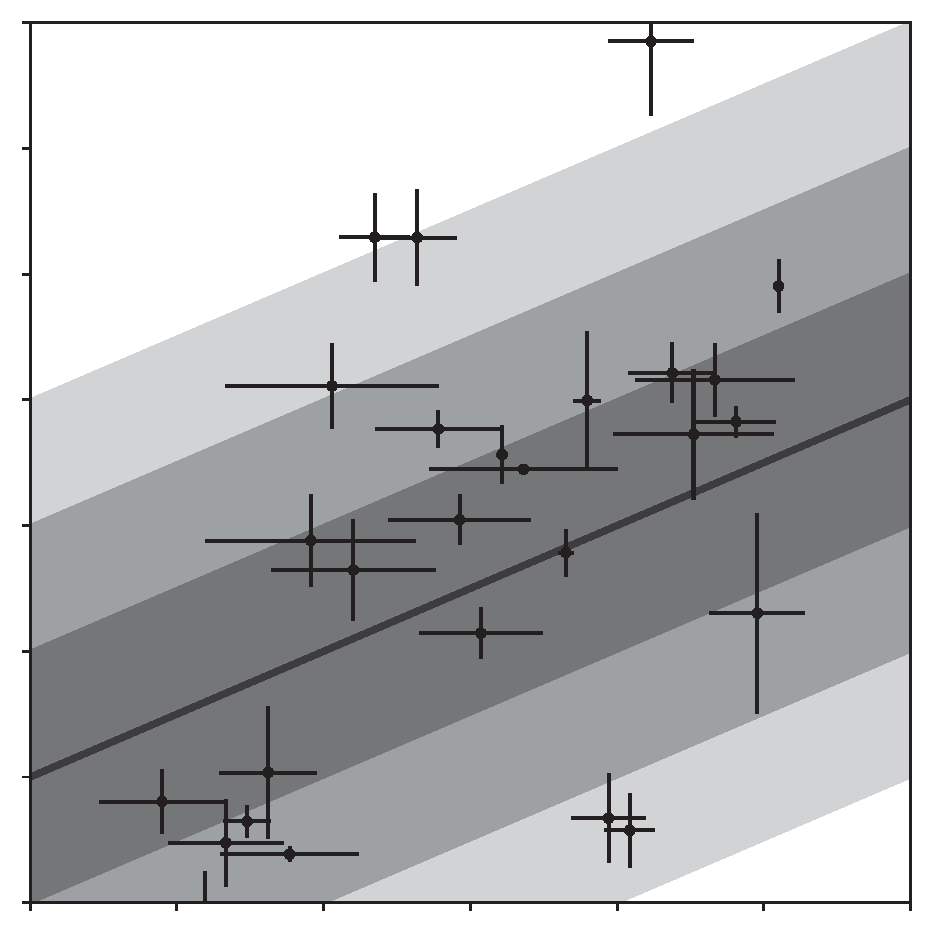
\includegraphics[width=0.8\linewidth]{figures/slopexample.eps}
    \caption{Example dataset and underlying model distribution where the scatter of the data cannot solely be accounted for by the error bars, which must be parameterized as extrinsic scatter, or \textit{slop}. Model distribution is shown with $1-$, $2-$ and $3\sigma$ confidence regions for the slop of the model, to properly account for the uncertainty in the dataset.}
    \label{fig:slopexample}
\end{figure}

In the following section, we will begin to explore how a likelihood function describing a model for this ``worst case'' type of dataset can be defined, by connecting the extrinsic and intrinsic probability distributions of the dataset with the model itself.

\subsection{The Likelihood Function}
The derivation below closely follows \textcite{trotter}, where the TRK statistic was initially formulated. In order to consider fitting a model to data, we must first determine how to quantify the goodness of fit for such a model, given some distribution of $N$ measurements described in the previous section. I define part of the model as some probability distribution $g(x,y)$ that is convolved along some model curve function $y_c(x;\vartheta_m)$, where $\vartheta_m$ is the set of parameters that define the functional form of the model; here, $g(x,y)$ can be thought of as the "density function" of the model distribution. Then, in order to properly represent the scatter of the data, I define the full model distribution by convolving this with a 2D Gaussian distribution that characterizes the slop, with widths defined by the parameters $\sigma_x$ and $\sigma_y$. This representation of the model can be difficult to conceptualize, but it is necessary in order to work with the most general, Bayesian treatment of a two-dimensional uncertain dataset. A visualization of this is shown in Figures \ref{fig:model} and \ref{fig:model_zoomedin}.

\begin{figure}
    \centering
    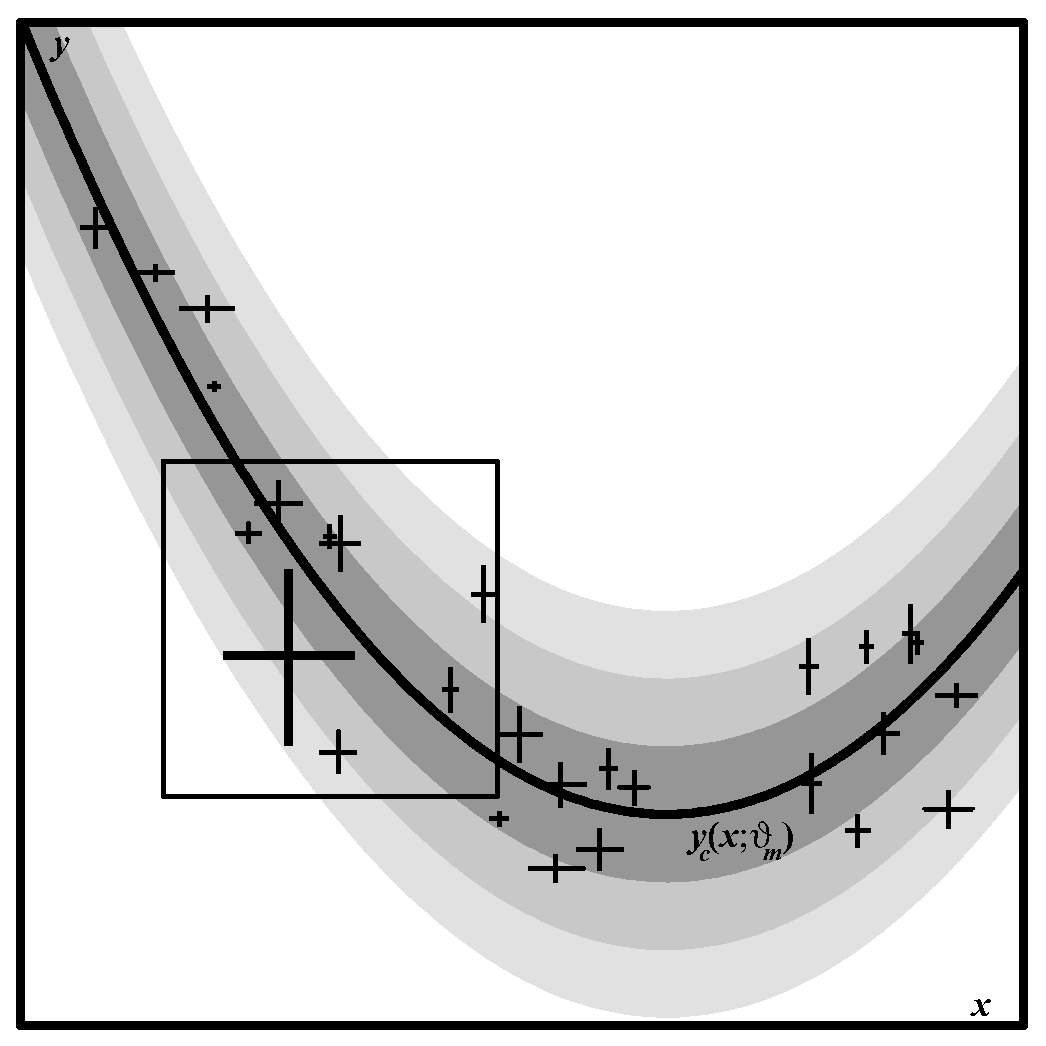
\includegraphics[width=0.8\linewidth]{figures/model.eps}
    \caption{Visualization of some two-dimensional dataset (from \textcite{trotter}) with both intrinsic and extrinsic scatter in two dimensions, and accompanying model distribution with $1-$, $2-$ and $3\sigma$ confidence regions for the extrinsic scatter/slop of the model represented by the shaded regions. Inset box is shown zoomed in Fig. \ref{fig:model_zoomedin}.}
    \label{fig:model}
\end{figure}

\begin{figure}
    \centering
    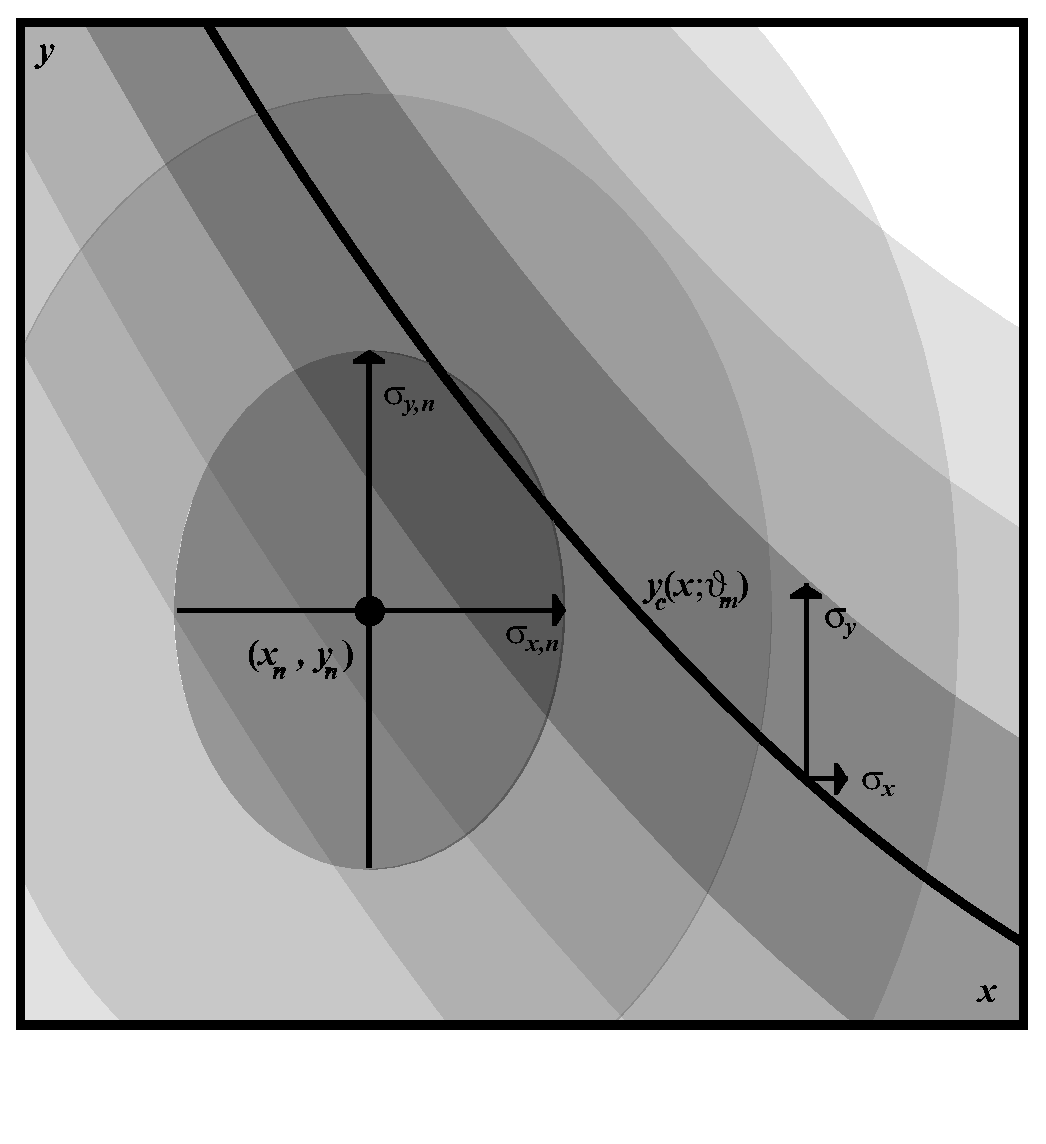
\includegraphics[width=0.8\linewidth]{figures/model_zoomedin.eps}
    \caption{Fig. \ref{fig:model}, zoomed in, from \textcite{trotter}. Centered is a single data-point $(x_n, y_n)$ with intrinsic probability distribution defined by its' error bars/intrinsic scatter $\sigma_{x,n}, \sigma_{y,n}$, alongside a model distribution with curve $y_c(x;\vartheta_m)$ and extrinsic scatter/slop parameters $(\sigma_x,\sigma_y)$. The shaded regions represent the $1-$, $2-$ and $3\sigma$ confidence regions of the datapoint's intrinsic probability distribution, and of the extrinsic scatter-convolved model distribution.}
    \label{fig:model_zoomedin}
\end{figure}

Another way to express the (effectively 1D) model curve $y_c(x;\vartheta_m)$ is do describe it as a one-dimensional delta function along some arbitrary chosen (orthogonal) coordinate system $(u_n, v_n)$. Indicated by the subscripts of $n$, such coordinates can, in the most general case, \textit{vary between datapoints}. As such, we can express the probability density along the model curve as $g(x,y)\delta(v_n, v_{c,n}(u_n;\vartheta_m))$, where $v_{c,n}(u_n;\vartheta_m)$ is $y_c(x;\vartheta_m)$ in the $(u_n, v_n)$ coordinate system, and $\delta$ denotes the one-dimensional Dirac delta function. Also note that given that the coordinates $(u_n, v_n)$ are assumed to be orthogonal, we can always express them as a rotation from $(x,y)$.

Now that we have an expression for the probability density along the model curve, we can convolve this with the extrinsic scatter/slop distribution (again, assumed to be 2D Gaussian) to obtain the \textit{model distribution function} for a single datapoint,
\begin{equation}\label{eq:pnmod}
    p_n^\text{mod}(x',y'|\vartheta_m,\sigma_x,\sigma_y)=\displaystyle\int_{u_n}\int_{v_n}g(x,y)\delta(v_n, v_{c,n}(u_n;\vartheta_m))\mathcal{N}(x'|x,\sigma_x)\mathcal{N}(y'|y,\sigma_y)\diff v_n\diff u_n,
\end{equation}
given the definition of the convolution of two bivariate functions, where the integrals are both over $(-\infty,\infty)$ and $\mathcal{N}$ denotes the Gaussian/normal distribution
\begin{equation}
\label{eq:symnorm}
    \mathcal{N}(x'|\mu,\sigma) = \frac{1}{\sqrt{2\pi\sigma^2}}\exp\left(-\frac{1}{2}{\frac{(x'-\mu)^2}{\sigma^2}}\right).
\end{equation}
with mean $\mu$ and standard deviation $\sigma$.

Next, we need to obtain an expression for the full \textit{joint} probability of a single datapoint with the model distribution function $p_n^\text{mod}$ for that datapoint. The \textit{intrinsic} probability for a single datapoint comes from the error bars for that datapoint, and is found with
\begin{equation}\label{eq:pnint}
    p_n^\text{int}(x',y'|x_n,y_n,\sigma_{x,n}, \sigma_{y,n}) = \mathcal{N}(x'|x_n,\sigma_{x,n})\mathcal{N}(y'|y_n,\sigma_{y,n}).
\end{equation}
again assuming Gaussian error bars. From here, we can find the joint probability of some $n^\text{th}$ datapoint with the model distribution by integrating the product of the two distributions $p_n^\text{mod}$ and $p_n^\text{int}$ over $x'$ and $y'$, as
\begin{align}\label{eq:pn}
p_n(\vartheta_m,\sigma_x,\sigma_y|x_n,y_n,\sigma_{x,n},\sigma_{y,n}) &= \nonumber
\int_{x^\prime}\int_{y^\prime}\int_{u_n}\int_{v_n}{g(x,y)\delta(v_n-v_{c,n}(u_n;\vartheta_m))} \times \nonumber \\
\mathcal{N}(x'|x,\sigma_x)\mathcal{N}(y'|y,\sigma_y)&\mathcal{N}(x'|x_n,\sigma_{x,n})\mathcal{N}(y'|y_n,\sigma_{y,n})\diff v_n \diff u_n \diff y^\prime \diff x^\prime \, .
\end{align}

Next, the likelihood function is defined to be the product of all $N$ of the joint probabilities of the datapoints, as
\begin{equation}\label{eq:likelibasic}
    \mathcal{L}=\prod\limits_{n=1}^Np_n(\vartheta_m,\sigma_x,\sigma_y|x_n,y_n,\sigma_{x,n},\sigma_{y,n}),
\end{equation}
so in theory, our work of finding an expression for the likelihood is done. However, given the four integrals in Equation \eqref{eq:pn}, this solution is quite computationally intractable. In order to obtain a practical likelihood, a few simplifying, but reasonable approximations need to be made, following \textcite{trotter}.

\subsection{An Analytical Approximation of the Likelihood}
\label{sec:tgtpts}
To begin, we can simplify the expression for the joint probability $p_n$ by noting that the $(x',y')$ integral in Equation \eqref{eq:pn} can be evaluated analytically, which gives
\begin{align}\label{eq:pnsimp}
& p_n(\vartheta_m,\sigma_x,\sigma_y|x_n,y_n,\sigma_{x,n},\sigma_{y,n}) = \nonumber\\
& \int_{u_n}\int_{v_n}{g(x,y)\delta(v_n-v_{c,n}(u_n;\vartheta_m))}\mathcal{N}(x|x_n,\Sigma_{x,n})\mathcal{N}(y|y_n,\Sigma_{y,n})\diff v_n \diff u_n \,,
\end{align}
where $(\Sigma_{x,n}, \Sigma_{y,n})$ are the quadrature sums of both the intrinsic and extrinsic scatters:
\begin{align}\label{eq:bigsigs}
\Sigma_{x,n} & \equiv \left( \sigma_{x,n}^2 + \sigma_x^2 \right)^{1/2} \nonumber\\
\Sigma_{y,n} & \equiv \left( \sigma_{y,n}^2 + \sigma_y^2 \right)^{1/2} \, . 
\end{align}
What is the significance of these terms? In the words of \textcite{trotter}, Equation \eqref{eq:pnsimp} indicates that the joint probability of some $n^\text{th}$ datapoint with the model distribution is proportional to the integral of the effectively one-dimensional probability density along the model curve through a two dimensional \textit{convolved} Gaussian, whose widths are the quadrature sums of the intrinsic and extrinsic uncertainties in each direction, $\Sigma_{x,n}$ and $\Sigma_{y,n}$. In other words, Fig. \ref{fig:model_zoomedin} is equivalent to \ref{fig:datapoint}.

\begin{figure}
    \centering
    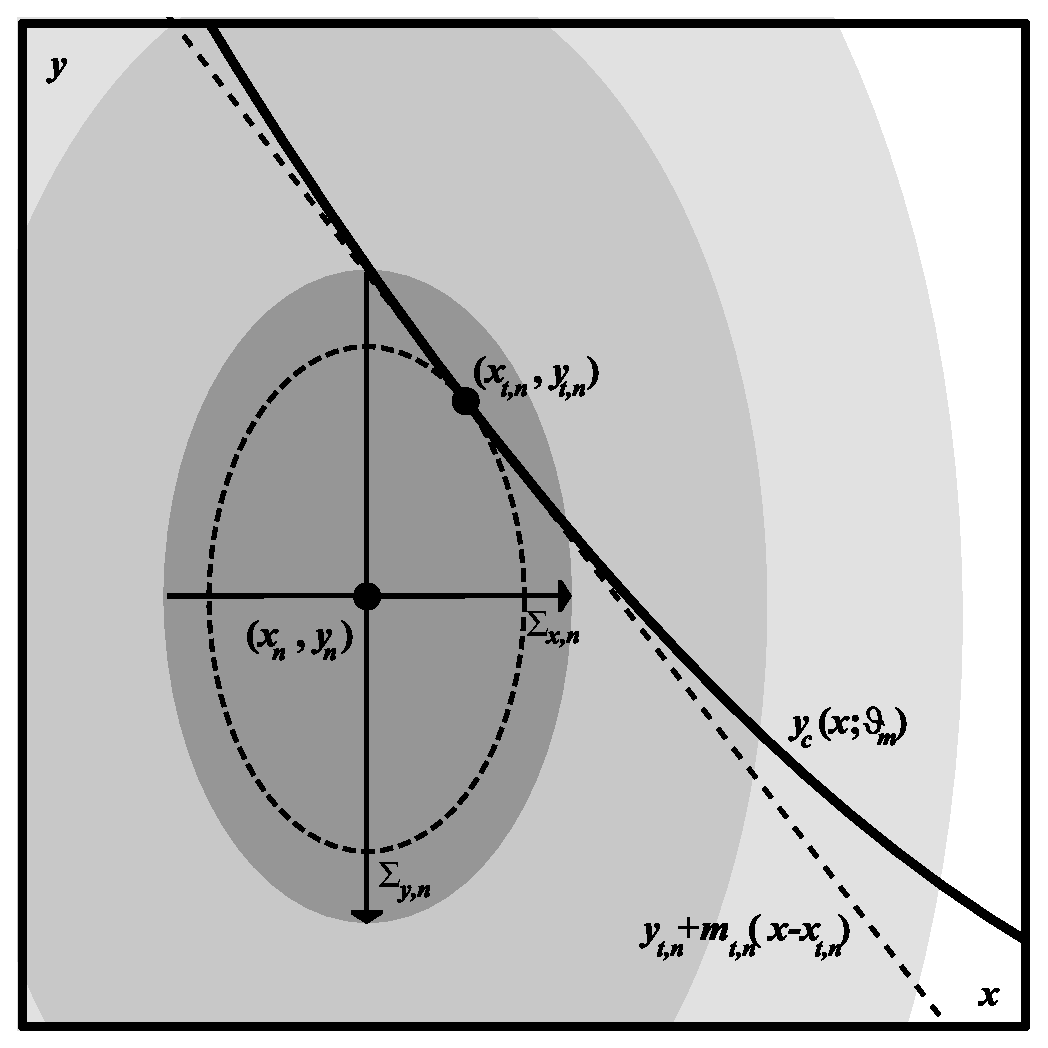
\includegraphics[width=0.8\linewidth]{figures/datapoint.eps}
    \caption{Visualization of some datapoint $(x_n,y_n)$ with convolved error ellipse defined by the extrinsic-intrinsic convolved error bars $(\Sigma_{x,n},\Sigma_{y,n})$, alongside some model curve $y_c(x)$. Also shown is the approximation of the non-linear model as a line tangent to the error ellipse at point $(x_{t,n},y_{t,n})$.}
    \label{fig:datapoint}
\end{figure}

To further simplify Equation \eqref{eq:pnsimp} (i.e., remove the integrals), I'll begin by making the first approximation: that the intrinsic probability density along the model curve $g(x,y)$ varies slowly with respect to the scale of the size of the convolved error ellipse described by $\Sigma_{x,n}$ and $\Sigma_{y,n}$. This will make $g(x,y)$ approximately constant, such that it can be pulled out of the integral in Equation \eqref{eq:pnsimp}. Next, I will assume that the model curve $y_c(x;\vartheta_m)$ is approximately linear over this same scale; specifically, I will approximate $y_c$ as a line $y_{t,n}(x)$ passing through the point $(x_{t,n},y_{t,n})$ where $y_c$ is tangent to the convolved error ellipse, with some slope $m_{t,n}$ (see Fig. \ref{fig:datapoint}), i.e.
\begin{equation}\label{eq:yclin}
    y_c(x)\approx y_{t,n} + m_{t,n}(x-x_{t,n}).
\end{equation}

If, at some position $x$, the model curve $y_c(x;\vartheta_m)$ is tangent to the error ellipse at some $(x_{t,n},y_{t,n})$, then we have the relation 
\begin{equation}\label{eq:tpoint1}
\frac{(y_c(x;\vartheta_m)-y_n)^2}{\Sigma_{y,n}^2}+\frac{(x-x_n)^2}{\Sigma_{x,n}^2} =  \frac{(y_{t,n}-y_n)^2}{\Sigma_{y,n}^2}+\frac{(x_{t,n}-x_n)^2}{\Sigma_{x,n}^2}\, ,
\end{equation}
which is the condition for $(x, y_c(x;\vartheta_m))$ to be a tangent point. Differentiating this equation with respect to $x$ gives
\begin{equation}\label{eq:tpoint2}
\dv{}{x}\left({\frac{(y_c(x;\vartheta_m)-y_n)^2}{\Sigma_{y,n}^2}+\frac{(x-x_n)^2}{\Sigma_{x,n}^2}}\right)=0 \, ,
\end{equation}
which implies that the tangent point is equivalent to the point on $y_c$ that \textit{minimizes the radial distance} to the centroid of the error ellipse. Evaluating the derivative gives us an equation that can be \textit{implicitly} solved for $x=x_{t,n}$,
\begin{equation}\label{eq:tpoint}
(y_c(x)-y_n)\dv{y_c(x;\vartheta_m)}{x}\Sigma_{x,n}^2+(x-x_n)\Sigma_{y,n}^2 = 0 \, ,
\end{equation}
given some model curve and datapoint.%\footnote{The actual method used to solve for these tangent points is covered in \S\ref{cha:code}.}.% For non-monotonic curves, there may be multiple such tangent points for a given datapoint; in this case, we take the tangent point that maximizes the joint probability.

Finally, given these two assumptions, the joint probability of the $n^\text{th}$ datapoint and the model distribution of Equation \eqref{eq:pnsimp} can be simplified by integrating over $v_n$, as
\begin{align}\label{eq:pnappint}
p_n(\vartheta_m,\sigma_x,\sigma_y|x_n,y_n,\sigma_{x,n},\sigma_{y,n}) \approx g(x_n,y_n)\int_{-\infty}^{\infty}{\mathcal{N}(x|x_n,\Sigma_{x,n})\mathcal{N}(y_c(x;\vartheta_m)|y_n,\Sigma_{y,n})\diff u_n}\, ,
\end{align}
given the ``selecting'' property of the delta function on the Gaussian along $y$. By using the chain rule substitution $\diff u_n = \dv{u_n}{x}\diff x$, $y_c(x;\vartheta_m)\approx y_{t,n}+m_{t,n}(x-x_{t,n})$ from Equation \eqref{eq:yclin}, and integrating over $x$, we have finally arrived at an analytic expression for $p_n$:\footnote{Here, we have also implicitly made an additional approximation: that the efficiency of which the measured data samples the \textit{true} model distribution is approximately constant along the scale(s) of $(\sigma_{x,n}, \sigma_{y,n})$ and $(\sigma_x,\sigma_y)$. This is unnecessary to delve into for the purposes of this work, but for an explicit inclusion of this, see \S2.2.1 of \textcite{trotter}.} 
\begin{align}\label{eq:pnanaly}
&p_n(\vartheta_m,\sigma_x,\sigma_y|x_n,y_n,\sigma_{x,n},\sigma_{y,n}) \\ &\approx g(x_n,y_n)\dv{u_n}{x}\mathcal{N}\left(y_n\left|\right.y_{t,n}+m_{t,n}(x_n-x_{t,n}),\sqrt{m_{t,n}^2\Sigma_{x,n}^2+\Sigma_{y,n}^2}\,\right) \nonumber \, .
\end{align}

The likelihood function is the joint probability of the model distribution with all of the datapoints, and the \textit{best fit} model parameters are defined as the parameters that, when plugged into the likelihood, maximize it. In other words, the likelihood is the product of all $N$ of the individual datapoints' joint probability distributions. In practice, rather than choosing to \textit{maximize} $\mathcal{L}$ to determine the best fit, it is much more common to \textit{minimize} $-2\ln\mathcal{L}$ (or some proportion thereof) in order to determine the best fit model parameters, for reasons of computational flexibility. In the simplifying ``traditional'' case of no error bars in $x$ and no slop whatsoever, $-2\ln\mathcal{L}$ is equivalent to the $\chi^2$ ``goodness-of-fit'' statistic, $\chi^2=\sum\limits_{n=1}^N\left[(y - y_c(x;\vartheta_m))/\sigma_{y,n}\right]^2$. As such, in our general case, $-2\ln\mathcal{L}$ is analogous to $\chi^2$, and has the form of
\begin{align}\label{eq:likegen}
-2\ln\mathcal{L} &= -2\sum_{n=1}^{N}{\ln p_n(\vartheta_m,\sigma_x,\sigma_y|x_n,y_n,\sigma_{x,n},\sigma_{y,n})} \nonumber \\
&=\sum_{n=1}^{N}\frac{\left[y_n-y_{t,n}-m_{t,n}(x_n-x_{t,n})\right]^2}{m_{t,n}^2\Sigma_{x,n}^2+\Sigma_{y,n}^2} -2\sum_{n=1}^{N}\ln\left(\dv{u_n}{x}\frac{1}{\sqrt{m_{t,n}^2\Sigma_{x,n}^2+\Sigma_{y,n}^2}}\right) + C \, ,
\end{align}
following Equations \eqref{eq:likelibasic} and \eqref{eq:pnanaly}, where $C$ is a constant\footnote{The explicit form of the constant $C$ is given in \textcite{trotter}, which isn't necessary for the purposes of this paper, as constant offsets are arbitrary for the process of likelihood maximization.}.

Recall that the rotated coordinate system $(u_n, v_n)$ in which the 1D model curve $\delta(v_n, v_{c,n}(u_n;\vartheta_m))$ is defined can be chosen at will, including the usage of different coordinates for different datapoints. As will be described in \S\ref{sec:compare}, different choices of these coordinates/of $\dv{u_n}{x}$ will give different statistics, with noticeably different properties. The following section will show how a certain choice of these coordinates will lead to the TRK statistic.

\subsection{The TRK Likelihood}
\label{sec:likelihood}
As shown in Equation \eqref{eq:likegen}, The arbitrary choice of the rotated coordinates $(u_n,v_n)$ and therefore the factor $\dv{u_n}{x}$ will be what defines a given statistic. While various choices for $\dv{u_n}{x}$ that lead to different statistics with different properties will be explored in \S\ref{sec:compare}, for now I will only examine the choice that leads to the TRK statistic, which is advantageous over other such statistics for reasons that will be addressed in \S\ref{sec:compare}.

The TRK statistic is defined such that for some $n^\text{th}$ datapoint, $u_n$ is chosen to be perpendicular to the line segment connecting the centroid of the datapoint $(x_n,y_n)$ with the tangent point $(x_{t,n},y_{t,n})$ discussed in the previous section. This choice results in a likelihood of the form
\begin{align}\label{eq:TRK}
\mathcal{L}^{\mathrm {TRK}} & \propto \prod_{n=1}^{N}{ \sqrt{\frac{m_{t,n}^2\Sigma_{x,n}^2+\Sigma_{y,n}^2}{m_{t,n}^2\Sigma_{x,n}^4+\Sigma_{y,n}^4}}\exp\left\{{-\frac{1}{2}\frac{\left[y_n-y_{t,n}-m_{t,n}(x_n-x_{t,n})\right]^2}{m_{t,n}^2\Sigma_{x,n}^2+\Sigma_{y,n}^2}}\right\}} \nonumber \\ -2\ln\mathcal{L}^{\mathrm{TRK}} &= \sum_{n=1}^{N}{\frac{\left[y_n-y_{t,n}-m_{t,n}(x_n-x_{t,n})\right]^2}{m_{t,n}^2\Sigma_{x,n}^2+\Sigma_{y,n}^2}} - \sum_{n=1}^{N}{\ln\left(\frac{m_{t,n}^2\Sigma_{x,n}^2+\Sigma_{y,n}^2}{m_{t,n}^2\Sigma_{x,n}^4+\Sigma_{y,n}^4}\right)} + C \, ,
\end{align}
which is the central equation of this work. One important property of the TRK statistic is that \textit{it is essentially a one-dimensional $\chi^2$-like statistic that is measured in the direction of the tangent point}\footnote{The derivation of this is beyond the scope of this work, but is found in \textcite{trotter}.}. For a visualization of the geometry of the TRK statistic, see Figure \ref{fig:datapointcolor}. Hereafter, I will sometimes use the shorthand  $\chi^2_\text{TRK}\equiv-2\ln\mathcal{L}^\text{TRK}$, especially in Chapter \ref{cha:code1} where it is frequently used.
% \begin{align}\label{eq:TRK}
% \mathcal{L}^{\mathrm {TRK}} & \propto \prod_{n=1}^{N}{ w_n\sqrt{\frac{m_{t,n}^2\Sigma_{x,n}^2+\Sigma_{y,n}^2}{m_{t,n}^2\Sigma_{x,n}^4+\Sigma_{y,n}^4}}\exp\left\{{-\frac{1}{2}w_n\frac{\left[y_n-y_{t,n}-m_{t,n}(x_n-x_{t,n})\right]^2}{m_{t,n}^2\Sigma_{x,n}^2+\Sigma_{y,n}^2}}\right\}}
% \end{align}

\begin{figure}
    \centering
    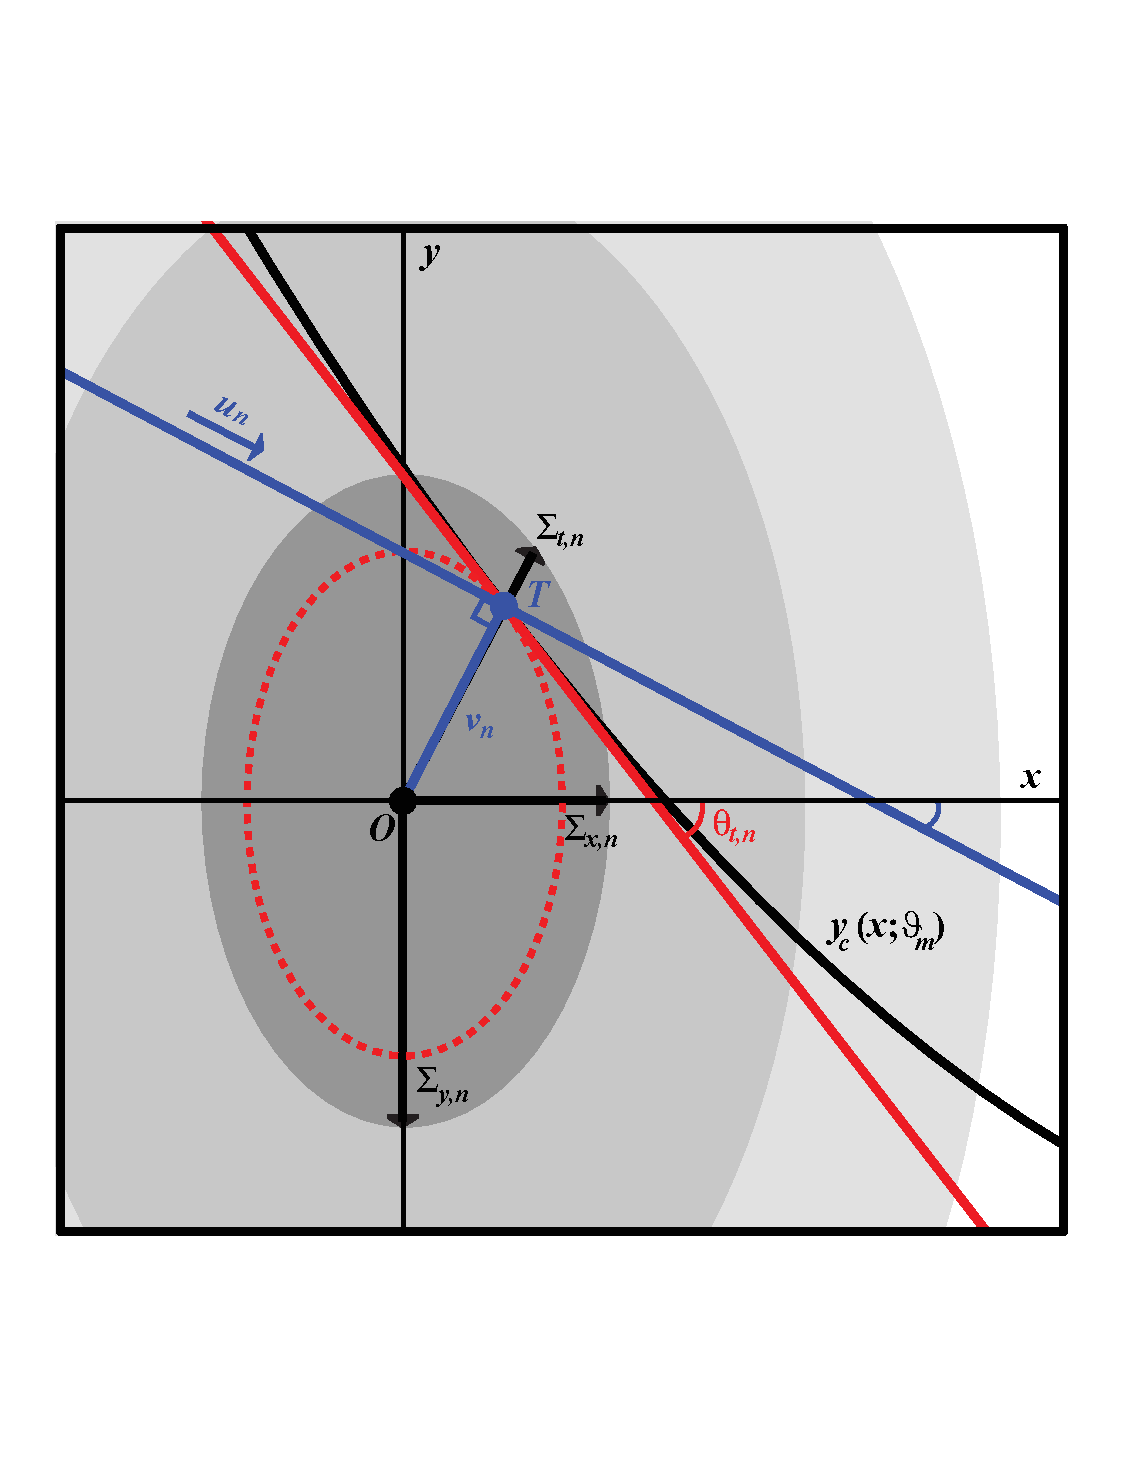
\includegraphics[width=0.8\linewidth]{figures/datapoint_med_simp.eps}
    \caption{Illustration of the geometry of the TRK statistic modified from \textcite{trotter}, given some datapoint and model. The datapoint is centered at $(x_n,y_n)$ (point $O$), with convolved error ellipse described by the widths $(\Sigma_{x,n},\Sigma_{y,n})$ (Equation \eqref{eq:bigsigs}). The model curve $y_c(x;\vartheta_m)$ is tangent to the convolved error ellipse at tangent point $(x_{t,n},y_{t,n})$ (point $T$), and the red line is the linear approximation of the model curve, with slope $m_{t,n}=\tan\theta_{t,n}$. The blue line indicates the rotated coordinate axis $u_n$ for the TRK statistic, perpendicular to the $v_n$ axis.}
    \label{fig:datapointcolor}
\end{figure}